%%----------------------------------------------------------------------
\subsubsection{Behavior Analysis of Taxi Drivers and Model Construction}
%% - - - - - - - - - - - - - - - - - - - - - - - - - - - - - - - - - - -

Real-life urban traffic flows consists of different types of vehicles, each of which has its own properties of behaviors. In the project, taxi is our primary target. 

We use probe-car data provided by a taxi company in Kyoto city for a one month period including approximately 700,000 location data points recorded per day.
%
In general, the driver’s behavior in VACANT state is driver-determined. That is, after dropping off passenger(s), a driver can freely select next destination and mode (queuing or cruising) for picking up the next passenger(s). In contrast, the destination in OCCUPIED state is passenger-determined. Given this fact, we hypothesize that the tendency of the location that a taxi driver got passenger(s) would be one of the main characteristics of the driver. For considering that, we focused on the preferred location to pick up passenger(s) and try to classified drivers based on that. 

\begin{figure}
  \centering
  \includegraphics[width=.9\linewidth]{Figs.hatto/fig-hatto-01.eps}
  \caption{Visualization of Origins for each Cluster : Red (High Ratio)⇔ Blue (Low Ratio)}
  \label{fig:Figs.hatto/fig-hatto-01.eps}
\end{figure}

To extract popular regions to get passenger(s), we apply kernel density analysis and the mean shift clustering algorithm which are widely used for extracting POI (Point of Interest) from the two-dimensional information provided by photo geo-tagging and GPS. From the results of Kernel density analysis, we can assume that the activity range defining the average driver’s interest point is 50 seconds of longitude and latitude.  We use these values as the bandwidth for the Mean-Shift clustering algorithm so that we got 15 regions. We then calculated the ratio of picking up passenger(s) at each region. We use the ratios and the affinity propagation clustering algorithm to classify all taxi drivers. This yielded 10 clusters of driver type.
\Figref{fig:Figs.hatto/fig-hatto-01.eps} shows the departure points for the clusters. These figures clearly indicate drivers tend to favor a specific territory for picking up passenger(s) . For example, 112 drivers for Cluster 1 tend to operate on the north side of Kyoto City. On the other hand, 33 drivers Cluster 4 are apt to go to the south side. 

\begin{figure}
  \centering
  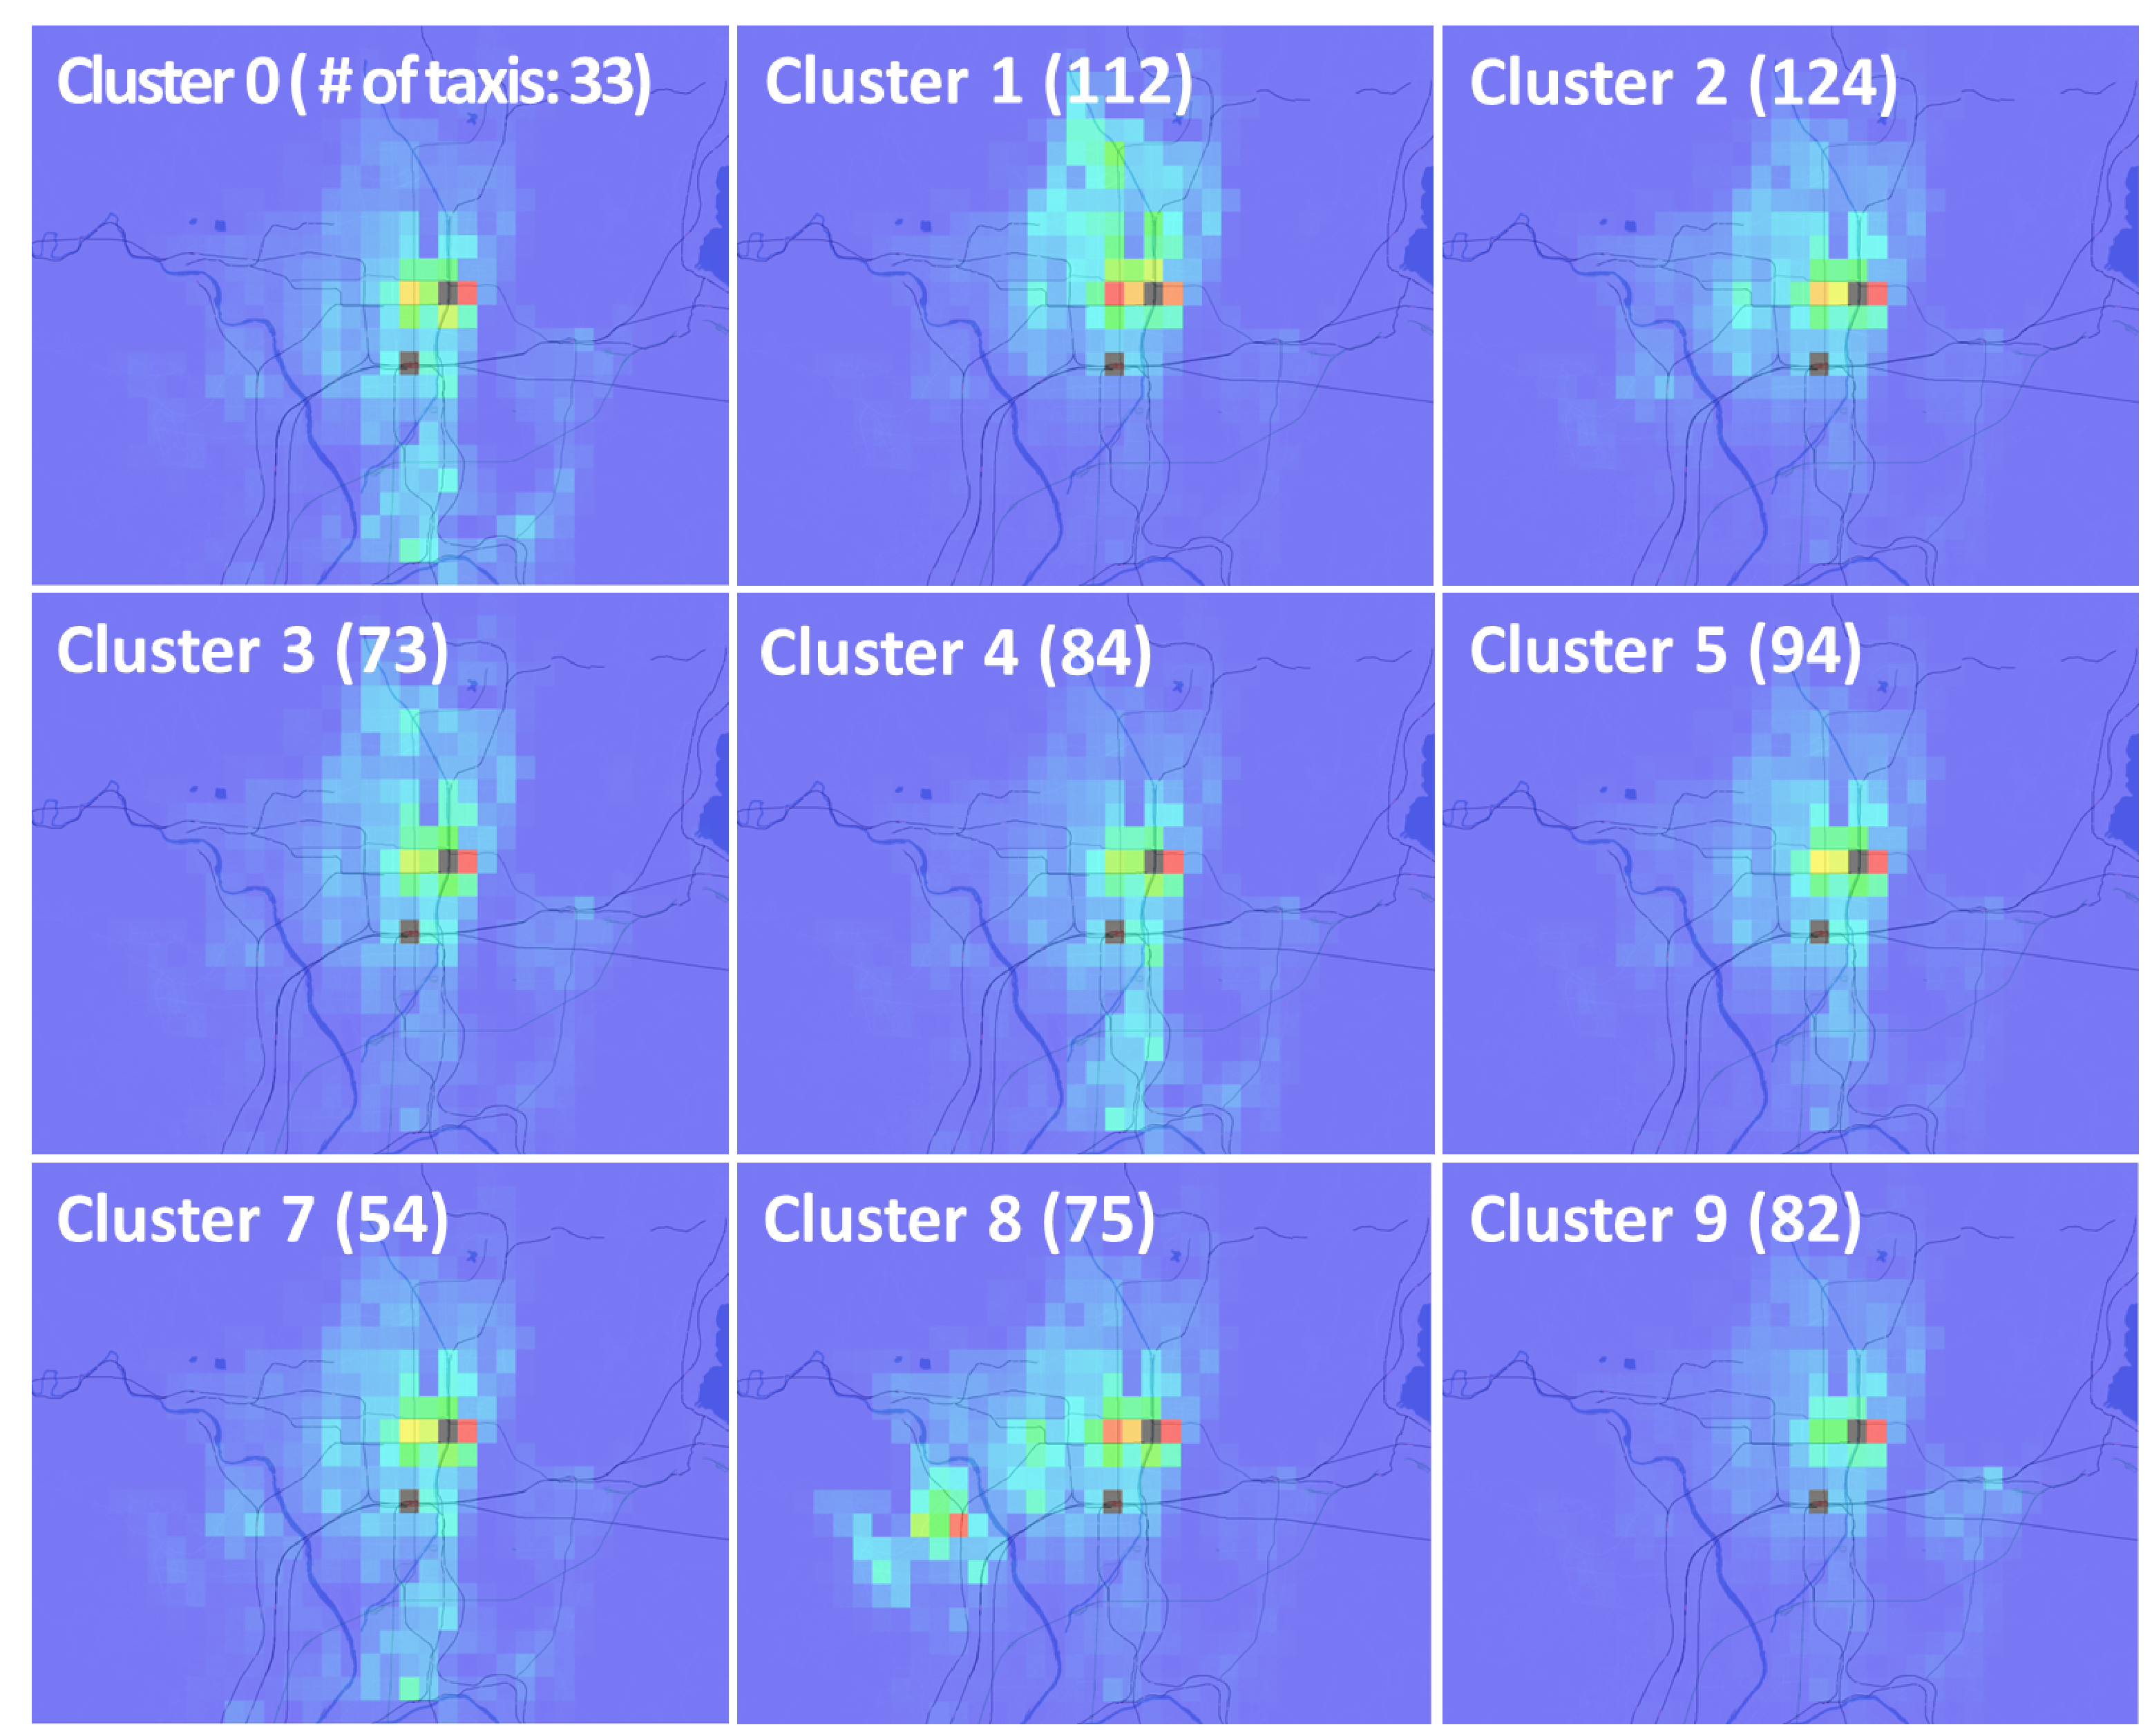
\includegraphics[width=.7\linewidth]{Figs.hatto/fig-hatto-02.eps}
  \caption{Comparison of Characteristic Behavior Model and Uniform Model}
  \label{fig:Figs.hatto/fig-hatto-02.eps}
\end{figure}

\begin{table}[]
\centering
\caption{Ratio of Staying Time in each Region}
\label{tbl:ratio-of-staying}
\begin{tabular}{|c|c|c|c|c|}
        \hline
        & \multicolumn{2}{|l|}{Probe-Data} & \multicolumn{2}{|l|}{Behavior Model} \\
        \hline
        & Cluster1       & Cluster4      & Cluster1         & Cluster4        \\
        \hline
Region3 & 0.263          & 0.056         & 0.217            & 0.095           \\
        \hline
Region4 & 0.016          & 0.196         & 0.054            & 0.165          \\
        \hline
\end{tabular}
\end{table}

In simulations each taxi agent has two states: OCCUPIED and VACANT. When the state changes from OCCUPIED to VACANT, taxi agents stochastically decide next destination and mode according to current time zone and current location. To analyze this decision-making process, we construct 10 driver models based on the clustering results shown in \figref{fig:Figs.hatto/fig-hatto-01.eps}. Further, if the taxi picks up a passenger(s) and changes their state to OCCUPIED, the destination is given by the passenger agent. Each passenger agent has an OD matrix whose contents stochastically mirror the probe-car data. In this taxi model, the driver type is given by 1) ratio of Queuing/Cruising, and 2) selection of area used in searching for passenger(s).
We conduct traffic simulations in the City of Kyoto with constructed taxi agents.
\Figref{fig:Figs.hatto/fig-hatto-02.eps} shows a visualization of agents whose model followed taxi driver cluster ID 1 or ID 4. ID 1 is a driver who tends to work in the northern part of Kyoto City while ID 4 is in the south. The characteristic behavior model confirmed that there is a deviation in the preferred areas for each taxi driver class as expected, see \figref{fig:Figs.hatto/fig-hatto-02.eps} (a) and (b). \Tabref{tbl:ratio-of-staying} lists the ratios of staying time in each region. Comparing probe-car data, it seems that the tendencies of agents follow the clustering result.
